\documentclass[submit, 12pt]{aiaa-pretty-modified}

\usepackage{graphicx}
\usepackage{array}
\usepackage{amsmath}
\usepackage{amssymb}
\usepackage{multirow}
\usepackage{rotating}
\usepackage[header,page]{appendix}
\usepackage{placeins}
\usepackage{pdfpages}
\usepackage[notbib]{tocbibind}
\usepackage{setspace}
\usepackage[tocindentauto]{tocstyle}

\usetocstyle{standard}


\newcommand{\Tablewidth}[0]{1in}
\newcommand{\Tablewidthtwo}[0]{3in}
\newcount\colveccount
\newcommand*\colvec[1]{
  \global\colveccount#1
  \begin{pmatrix}
    \colvecnext
  }
  \def\colvecnext#1{
    #1
    \global\advance\colveccount-1
    \ifnum\colveccount>0
    \\
    \expandafter\colvecnext
    \else
  \end{pmatrix}
  \fi
}


\begin{document}
\begin{titlepage}

\begin{center}

\vspace*{3cm}

\textsc{{\Huge Planning Algorithms for Indoor Robotic Odor Localization}}\\[3cm]

{\Large Final Report}\\
{\large 16.622}\\
{\large Fall 2012}\\
[1.5cm]

% \emph{Authors:}\\
% Troy \textsc{Astorino}\\
% Mark \textsc{Van de Loo}\\
% [1.5cm]

% \emph{Advisors:}\\
% Professor Youssef \textsc{Marzouk}\\
% Professor Nicholas \textsc{Roy}\\
% Josh \textsc{Joseph}\\
% Javier \textsc{Velez}\\
% Xun \textsc{Huan}\\
% Sachi \textsc{Hemachandra}

\emph{Authors:}\\
Troy Astorino\\
Mark Van de Loo\\
[1.5cm]

\emph{Advisors:}\\
Professor Youssef Marzouk\\
Professor Nicholas Roy\\
Josh Joseph\\
Javier Velez\\
Xun Huan\\
Sachi Hemachandra


\end{center}
\vfill

\today
\end{titlepage}

\newpage
\section*{Abstract}
A greedy gradient descent planning algorithm and a stochastic planning algorithm
were compared in the context of indoor robotic odor localization. A ground robot
was equipped with an electronic nose that uses metal oxide sensors to measure
chemical concentration. State estimation was implemented through the use of a
particle filter that assumed a chemical concentration profile exponentially
decaying with the square of the distance to the source. In localizing a single
chemical vapor source in a closed room, there was not shown to be a
statistically significant difference between the localization rates achieved by
the two planners. It is concluded that further research in the area of modeling
and estimation techniques for indoor robotic odor localization is necessary, and
potential directions for future work are discussed.


\newpage

\tableofcontents

\newpage

\listoffigures

\newpage

\listoftables

\newpage
\onehalfspace

\section{Introduction}

Robotic odor localization\footnote{Odor localization
  is defined as ``the act of finding the location of a
volatile chemical source in the environment.''\cite{kowadlo}} has real-world applications such as searching for a chemical leak in a
factory or laboratory, or locating survivors of a natural disaster
amidst the rubble of collapsed buildings.  These applications require an odor localization robot to operate autonomously
in an indoor environment.  Indoor air currents caused by
factors such as
ventilation and air circulation systems, moving people or machinery,
convection, and drafts from the outdoors represent a challenge in the
localization of a chemical vapor source,
since these effects may become dominant over diffusion and are unpredictable.

The purpose of this experiment was to explore the possibility of
utilizing a probabilistic approach to robotic odor localization to mitigate the uncertainty
introduced in the behavior of a chemical vapor plume by indoor
air currents.  Probabilistic approaches to robotic odor localization may be analyzed as a combination of
three components: a model, an estimator, and a planner. The model is a
mathematical function that describes the spatiotemporal variation of the
chemical concentration. The estimator represents the process by which
measurements of the chemical concentration are combined with model in real time
to obtain an estimate of the location of the chemical source. The planner is an
algorithm that decides the location of the next measurement given the current
estimate and confidence interval of the source location.

The goal of this experiment was to compare two different planners,
assuming a Gaussian model and a Bayesian inference estimator as
parameters of the experiment.  No statistically significant difference
was shown between the performance of the two planners compared.

\section{Hypothesis, Objective, Success Criteria}
\label{sec:hos}
\subsection*{Hypothesis} 
The mean localization rate of a 35-minute two-dimensional search by an
autonomous ground robot equipped with a chemical vapor sensor will be 20 percent
greater using a stochastic planner than using a simple gradient descent planner.
\footnote{ The simple gradient descent (also reffered to as greedy) algorithm always moves the robot in the
  direction of the best source estimate. A stochastic algorithm moves to a
  location randomly sampled from the source estimate probability distribution,
  allowing the planning algorithm to gain a more complete representation of the
  search space, at the potential cost of taking some unnecessary measurements.}

\subsection*{Objective}
Equip a ground robot furnished by the CSAIL Robust Robotics Group with an Alpha MOS NEEM chemical sensor, implement the planners on the robot's software platform, and assess the mean localization rate of a cup of ethanol in a closed room.

\subsection*{Success Criteria} 
Determine the difference in mean localization rate to a sufficient precision such that the hypothesis can be assessed.

\section{Literature Review}
\label{sec:lit-review}
Review of previous work in the field of robotic odor localization helped to select
this experiment's test environment of windless indoor rooms with uncommon
geometries. In addition, it provided the basis for the selection of a Bayesian inference
estimator and a Gaussian model as parameters of the experiment, and
motivated the selection of a simple gradient descent planner and a stochastic
gradient descent planner as interchangeable parts of the localization algorithm
to be compared for speed.

\subsection{Experiment Motivation}
Robotic odor localization experiments have been conducted using chemical
dispersion in water, air, and soil.\cite{kowadlo} In water and soil, diffusion is the
dominating method by which a chemical emanates from a source and disperses
through space. In air, where the Reynolds number is higher than in water or
soil, the behavior of the chemical concentration is affected by the presence of
turbulent fluid currents in addition to chemical diffusion.\cite{kowadlo} These turbulent
currents have led most robotic odor localization researchers to introduce an
artificial wind source when working in air. This negates the effect of the
turbulence, producing a concentration plume that behaves as a 2-dimensional
Gaussian function in planes normal to the wind direction, and downwind of the
source. \cite{ferri} While smoothing the concentration field in this manner makes the task of locating the
chemical source more straightforward, this environment is not representative of
a realistic indoor scenario. A few experiments, such as that done by Ferri, et
al., have been conducted in an indoor environment without an artificial wind
source. \cite{ferri} In general, however, it seems that turbulent indoor environments
have been less explored than their artificial wind source counterparts. For this
reason, it was decided that this experiment would be conducted in an ambient,
windless indoor environment.

\subsection{Selection of Model and Estimator}
Due to the varying effects of turbulence and diffusion discussed in section 3.1,
accurate modeling of the concentration field is dependent upon the medium and
environment in which the experiment is conducted. However, many robotic odor
localization researchers chose not to use a high-fidelity model of the
concentration field, deeming this level of complexity unnecessary. \cite{kowadlo} Most
commonly used was a dispersion model based on a Gaussian function. Time
invariant Gaussian models were used successfully in experiments in water and
soil, as well as in air with an artificial wind source. \cite{kowadlo} In turbulent air,
Ferri, et al. successfully used a time invariant monotonic function with a
single peak at the source location as a concentration model. \cite{ferri} The two
algorithms tested both successfully localized a dish of ethanol in a mean time
of less than 10 minutes, beginning an average distance of 1.8m from the source.
The model used in these localization algorithms is not explicitly described in
\cite{ferri}, but the assumption that the model is time invariant and monotonic with a
single peak is a defining component of the successful localization algorithms
presented in this paper. Based on the success of Ferri, et al., it was
deemed reasonable to choose a Gaussian model for this
experiment, and to treat
the effects of turbulent fluid currents in the air as noise. A Bayesian filter
was selected as an estimator to account for this noise in determining a
probability distribution of the source 
location after each measurement. The
Bayesian filter is a common technique used in conjunction with Gaussian models
in robotic localization and is described in \cite{bergman}.

\subsection{Selection of Planners}
Planners that were shown to be effective in turbulent air environments were
mainly derived from observations of the behavior of biological organisms.
\cite{ferri} For example, Ferri et al. attempted to mimic the circling behavior
of the Luna Moth in its search for a mate in one planner, and the weighted
random walk exhibited by the chemotaxis of the E. coli bacterium in another.
\cite{ferri} No documentation of simple gradient descent using a single sensor
or other simple statistically motivated planners as applied to robot odor
localization was found. Using simple gradient descent is attractive because of
its simplicity, but due to the turbulent nature of ambient indoor air, a simple
gradient descent planner may be prone to confusion by temporary local maxima of
the chemical concentration. An alternative planner that may perform better in
the turbulent environment without requiring a complicated model is based on
stochastic gradient descent, which adds randomness to the gradient vector when
prescribing the direction of motion. \cite{bottou} This randomness may
help avoid
the issues caused by temporary local maxima.

\section{Description of Experiment}
\subsection{Experimental Overview}
A greedy gradient descent planning aglorithm and a
stochastic planning algorithm were tested using the
same measurement model and estimation algorithm. A sensor capable of identifying the
concentration of ethanol in the surrounding air was mounted on a ground
robot. A dish of ethanol was placed in a test room, and the mean rate at which the robot localized the ethanol source
using the greedy planner was compared to the mean rate using the
stochastic planner.

\subsection{Test Apparatus}
\label{sec:design}
\subsubsection{Hardware and Robot Platform}

The Alpha MOS NEEM chemical sensor shown in Figure \ref{fig:sensor} was
attached to the Envoy robotic platform of the Robust Robotics Group, illustrated in Figure \ref{fig:wheelchair}.  The sensor was mounted
30 cm above the ground.


\begin{figure}
\begin{center}
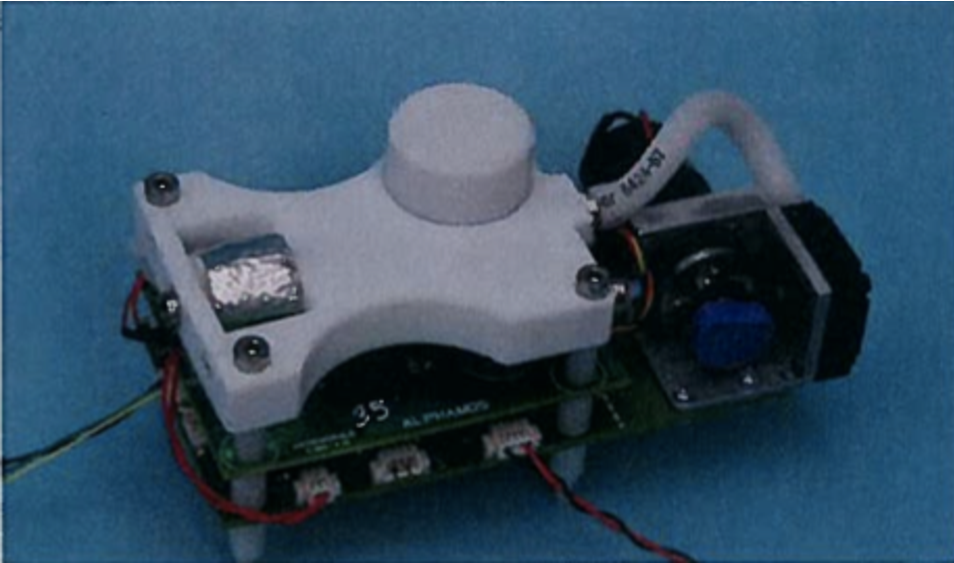
\includegraphics[width=3in]{img/sensor.pdf}
\caption{Alpha MOS NEEM chemical sensor.}
\label{fig:sensor}
\end{center}
\end{figure}

A laptop computer
mounted on the robot performed all real-time computation and data
collection.  The robot used two LIDARs and a pre-loaded map of the
test room to determine its position.  The robot's position was made available
as telemetry to the estimator via the LCM messaging protocol at a rate
of 40 Hz as
illustrated in Figure \ref{fig:acquisition}.

\begin{figure}
\begin{center}
\includegraphics[width=5in]{img/wheelchair.pdf}
\caption{Envoy robotic wheelchair platform with Alpha MOS Neem Sensor.}
\label{fig:wheelchair}
\end{center}
\end{figure}

\FloatBarrier

\label{sec:mount}

\subsubsection{System Control Flow}

After reaching each measurement location commanded by the planner, the robot
entered a waiting period of 30 seconds to allow transient concentration
behaviors and sensor dynamics to attenuate before beginning to take readings.
This period was followed by another 30 second period during which readings of
the chemical vapor concentration were recorded at a rate of 1 Hz. These readings
were averaged, and the natural logarithm of the average was passed to the
estimator. An average reading was used because it was observed that there was a
large variance in the readings measured at any given location, a variance on the
same order of magnitude as the average reading value. The estimator then used
this value and the current position of the robot to update its posterior belief.
This belief was passed to the planner, which commanded the next measurement
location to the robot. The robot moved to that location and began the process
again. Data flow between the components of the system is illustrated in Figure
\ref{fig:acquisition}.

\begin{figure}
\begin{center}
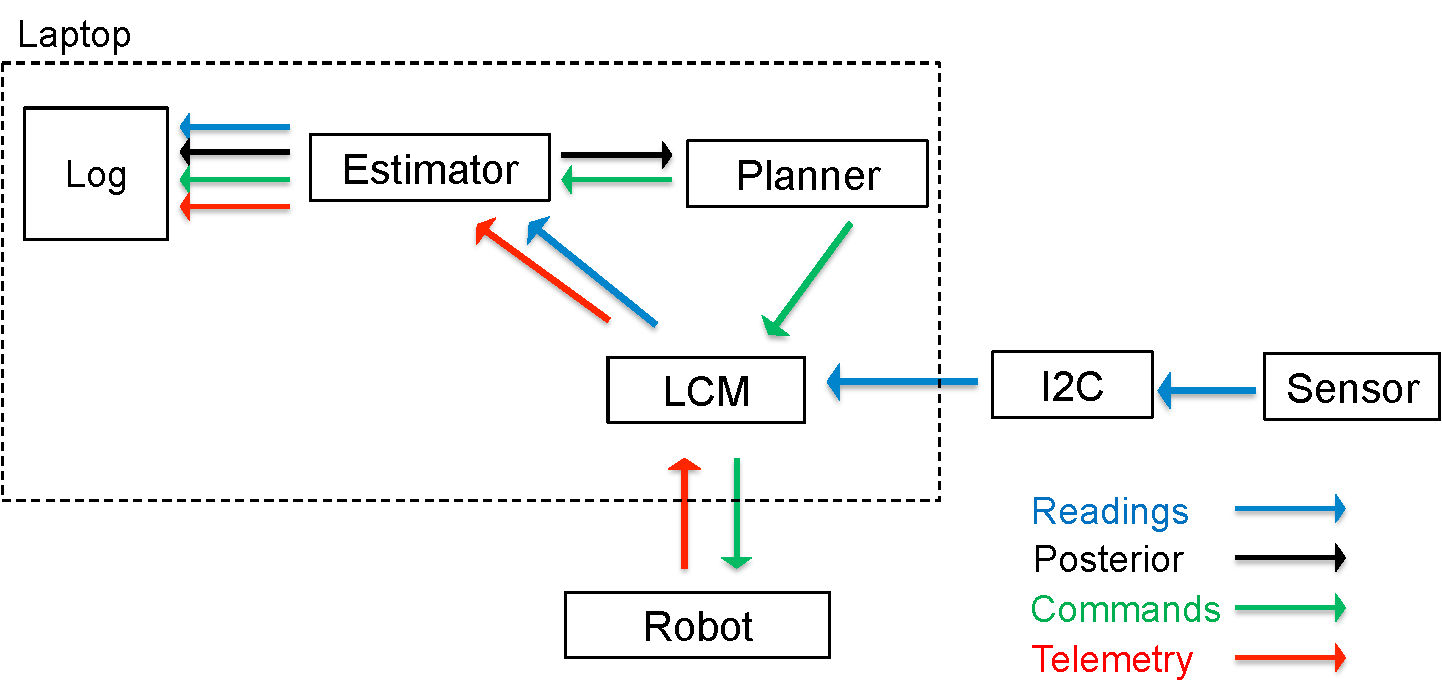
\includegraphics[width=6in]{img/acquisition.pdf}
\caption[Data acquisition flowchart]{The components of the system, and the paths along which data is
  communicated. Messages are passed among different components of the robot's
  software using the LCM protocol.  Sensor readings consist of a raw
  chemical concentration value.  The
  posterior distribution is the robot's current best estimate of the chemical
  source's location. Commands are sent in the form of a target position and
  orientation of the robot. Telemetry includes the robot's position, velocity,
  and attitude.}
\label{fig:acquisition}
\end{center}
\end{figure}

\subsubsection{Estimator}

The estimate of the source location was calculated using a particle
filter\cite{maskell2001tutorial}. The particles were distributed with uniform
spacing over the area of the test room, and each particle held the posterior
estimate's belief that it was the location of the source. The particle density
used is given in Table
\ref{tab:estimator-parameters}. 

Each time the estimator received a
measurement, a Bayesian update was performed on each particle
as follows: 
\[P_n(x_i = x_s) \propto P(c_n | x_i = x_s) P_{n-1}(x_s = x_i)\]
In the above expression, $P_n(x_i = x_s)$ represents the posterior belief that the source is located at the
$i^{th}$ particle location after the $n^{th}$ update.  $x_i$
represents the position of the $i^{th}$ particle, $x_s$ represents the
position of the source, and $c_n$ represents
the $n^{th}$ measurement received by the estimator. $P(c_n | x_i =
x_s)$ is the likelihood function, the probability that the measurement
is equal to $c_n$ given that the source is at the $i^{th}$ particle location according to
the measurement model. The measurement model is a normal
distribution of concentration
measurements according to: 
\[c \sim \mathcal{N}\left(\bar{c}(x_s,x_r), \sigma \right)\]
\[\bar{c}(x_s,x_r) = q \exp{\left[-\frac{|x_r - x_s|^2}{\nu^2}\right]} + k\]
where $x_r$ is the robot's location when the measurement is taken. The parameter
values $\sigma$, $q$ and $\nu$ were fitted from preliminary concentration data.
The preliminary data, alongside the fitted curves, is presented in Figure
\ref{fig:model-fit}, and the values resulting from this are shown in Table
\ref{tab:estimator-parameters}. Because the baseline chemical sensor reading was
observed to vary across the preliminary trials, the height offset $k$ was
calculated by measuring the average baseline sensor reading over 60 seconds
before the the trial began. The computed height offsets for each trial are listed in Table \ref{tab:height-offset}. 

This simple measurement model does not consider
asymmetric diffusion, time variation of diffusion, convection and wind currents,
or the dynamic response of the sensor, all of which may have been present as
disturbances in the test environment. It was believed that the estimation
technique would cause the posterior estimate to accurately converge to the true
source location by treating the deviations of real-world dynamics from the
simple model as measurement noise.

\begin{table}
\caption[Estimator parameters]{Particle filter and measurement model parameters.}
\begin{center}
\begin{tabular}{|c|c|}
\hline
Particle density & 69.4 $\frac{particles}{m^2}$ \\ \hline
$\sigma$ & 1.0 \\ \hline
$q$ & 0.3748 \\ \hline
$\nu$ & 1.085  \\ \hline
$k$ & -10.8534  \\ \hline
\end{tabular}
\end{center}
\label{tab:estimator-parameters}
\end{table}

\begin{figure}
\begin{center}
\fbox{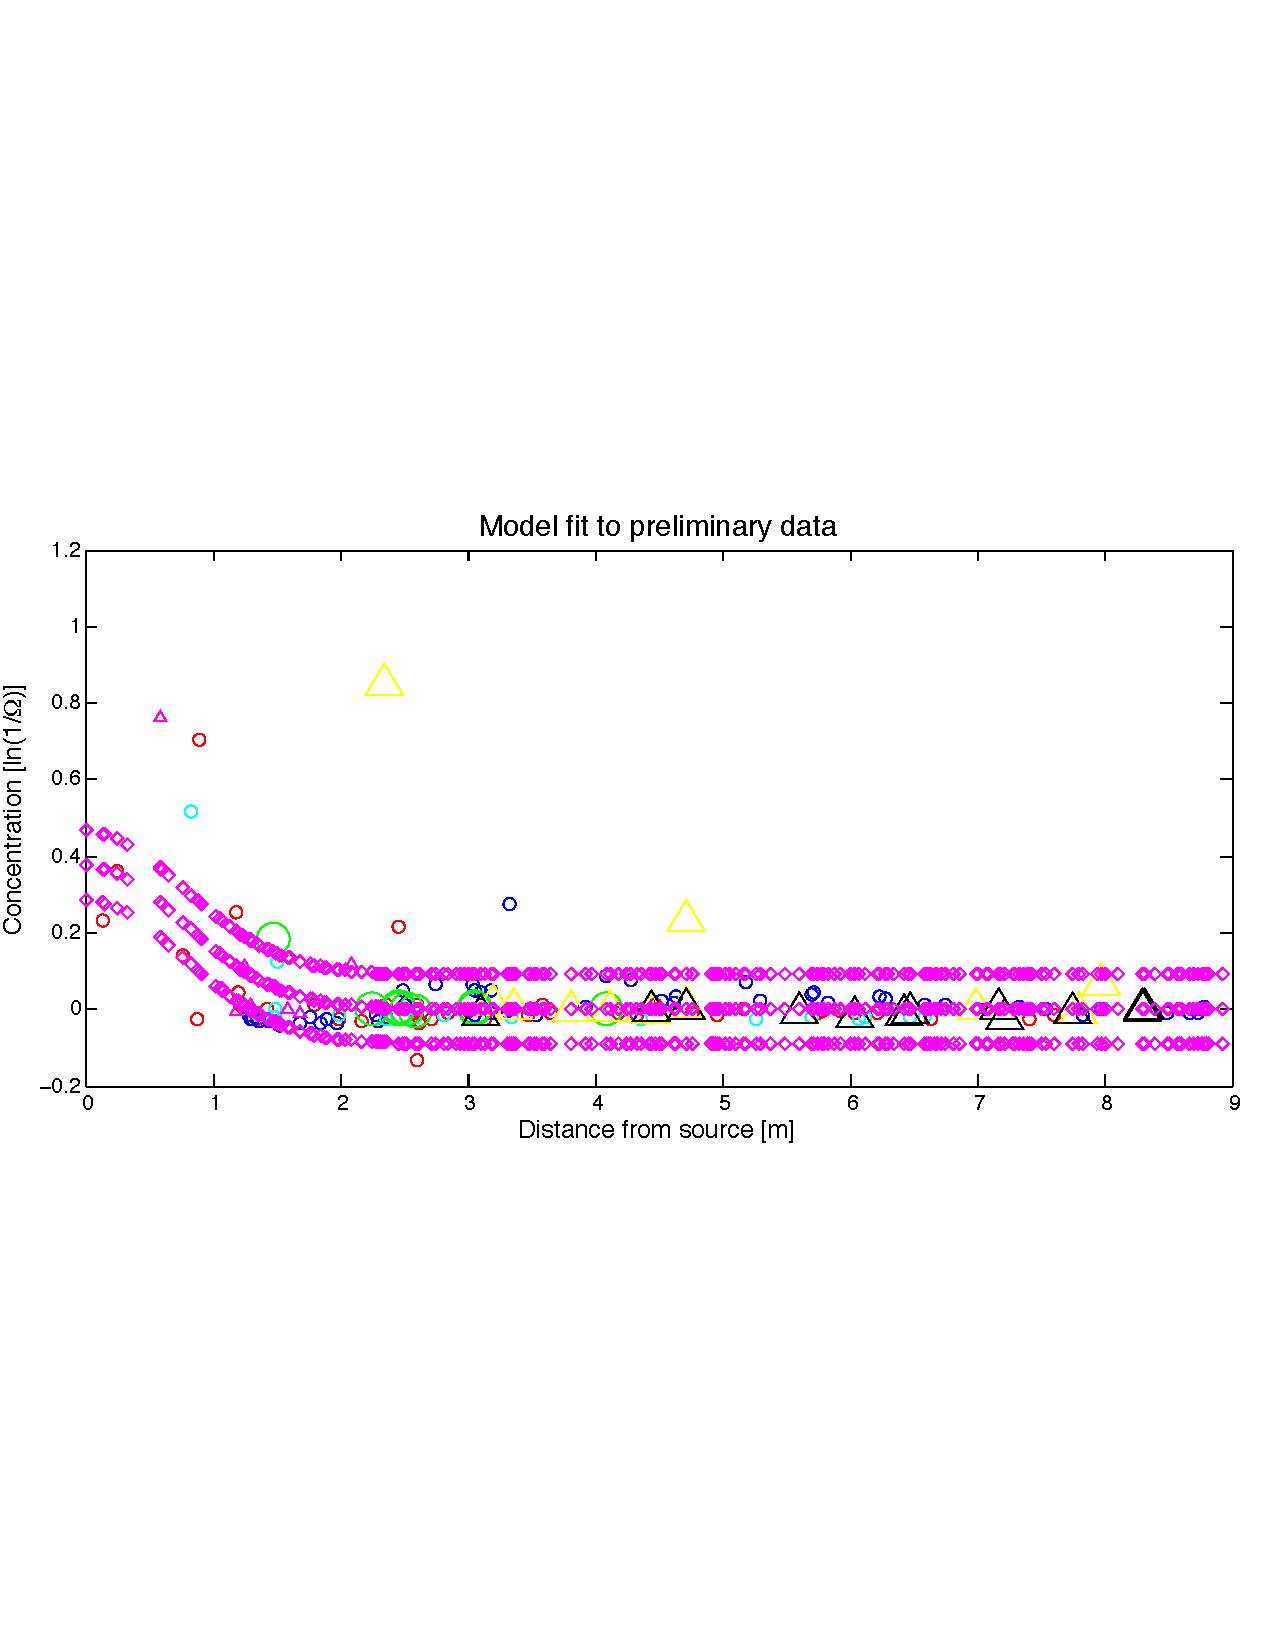
\includegraphics[width=6in]{img/model-fit.pdf}}
\caption[Fit of model parameters to preliminary data.]{
  The fit of the measurement model to preliminary data. The purple
  diamonds show measurement models for different sets of trial data. The Alpha
  Mos NEEM sensor had different baseline concentration values on different days,
  so the measurement model used a height offset dependent on the baseline
  concentration on a given day. The other markers represent actual measured
  concentrations. The markers that are the same shape and color are from the
  same trial.}
\label{fig:model-fit}
\end{center}
\end{figure}

\begin{table}
\caption{Measurement model height offsets.}
\centering
\resizebox{\columnwidth}{!}{
\begin{tabular}{|c||c||c||c||c||c||c||c||c||c|}
\hline
Height offset $k$ & 1 & 2 & 3 & 4 & 5 & 6 & 7 & 8 & 9 \\
\hline \hline
Greedy & -10.7078 & -10.8031 & -10.6224 & -10.8217 & -10.7253 & -10.5972 & -10.3781 & -10.5596 & -10.8351 \\
\hline
Stochastic & -10.7088 & -10.5289 & -10.7939 & -10.7022 & -10.7959 & -10.9099 & -10.4587 & -10.5746 & -10.9096 \\
\hline
\end{tabular}
}
\label{tab:height-offset}
\end{table}

\subsubsection{Planner}
This experiment compared a simple gradient
descent (greedy) planning algorithm and
a stochastic planning algorithm. The greedy algorithm always chose the
next measurement location 1.5 m away from the robot's current
position, in the direction of the maximum probability estimate of the source location. The
maximum probability estimate was calculated by taking the weighted average of
all of the estimator particle locations:
\[\hat{x_s} = \displaystyle\sum\limits_{i} x_i P(x_s = x_i) \]
The stochastic planner sampled a random particle from the posterior probability 
distribution of the estimator, and chose that particle's location as
the next measurement location.  After choosing the next measurement
location, the planner commanded the robot to move to that location.


% \begin{table}
% \caption{Planner parameters}
% \begin{center}
% \begin{tabular}{|p{\Tablewidthtwo}|p{\Tablewidthtwo}|}
% \hline
% Commanded movement distance for greedy algorithm & 1.5 $m$ \\ \hline
% Time to wait for air to settle & 30 $sec$ \\ \hline
% Time to take readings &  30 $sec$ \\ \hline
% \end{tabular}
% \end{center}
% \label{tab:planner-parameters}
% \end{table}

\subsection{Experimental Process}
\subsubsection{Test Environment}

The experiment was conducted in a single test room with a floorplan
shown in Figure \ref{fig:testroom}. The ventilation system of the room was undisturbed in order to keep the test
environment close to that of a typical indoor environment. Parameters of the
experiment are shown in Table \ref{tab:parameters}.

\begin{figure}
\begin{center}
\fbox{
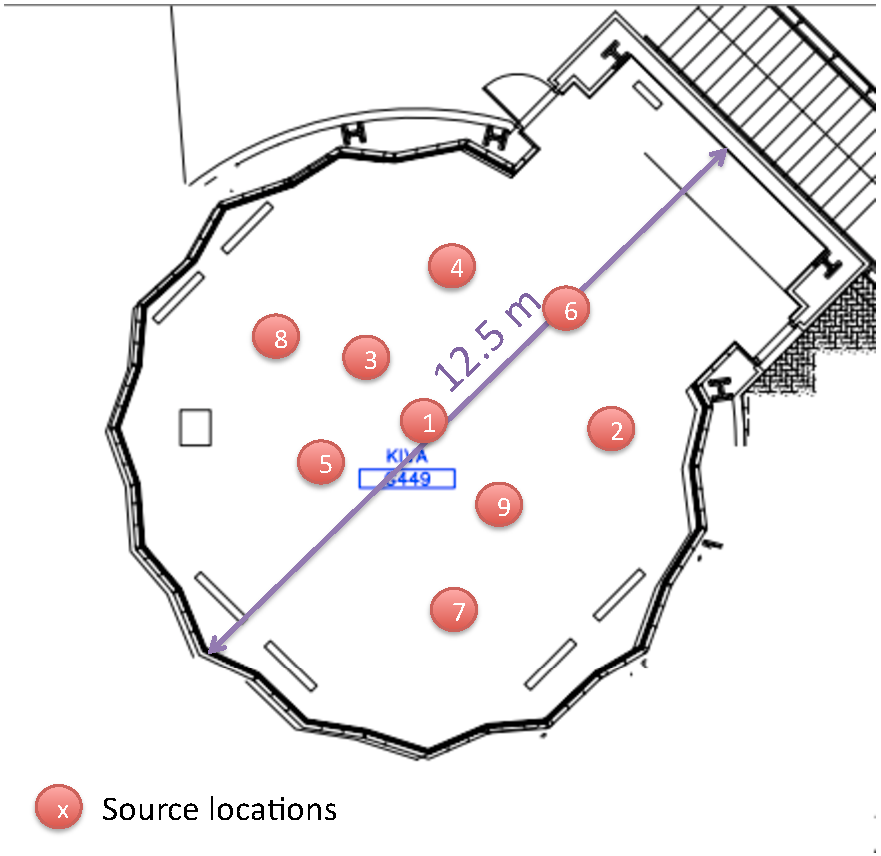
\includegraphics[width=4in]{img/testroom.pdf}}
\caption{Testroom floorplan and chemical vapor source locations.}
\label{fig:testroom}
\end{center}
\end{figure}

\begin{table}
\caption{Parameters of the experiment.}
\begin{center}
\begin{tabular}{|p{\Tablewidthtwo}|p{\Tablewidthtwo}|}
\hline
Chemical used as source & Liquid ethanol, 70\% \\ \hline
Surface area of chemical vapor source & 0.018 $\text{m}^2$\\ \hline
Vertical distance between sensor plane and
test room floor & 0.3 $\text{m}$ \\ \hline
Minimum initial distance between sensor and chemical & 2 $\text{m}$ \\ \hline
Delay between robot start and source exposure & 30 minutes \\ \hline
Delay between source exposure and the start of a trial & 30 minutes \\ \hline
Duration of trial & 35 minutes \\ \hline
\end{tabular}
\end{center}
\label{tab:parameters}
\end{table}

\subsubsection{Test Procedure}
A single exposed dish of ethanol was placed in the test room at least 30
minutes before the start of each trial, and remained undisturbed at
its initial location for the entirety of the trial. The robot was
initialized at a random location no less than 2 meters away from the
location of the source, and operated  autonomously throughout
the trial.  The duration of each trial was 35 minutes, beginning when
the first chemical sensor reading was taken. 

Nine sets of two trials were conducted using the nine chemical source
locations shown in Figure \ref{fig:testroom}.  For each source
location, one trial was conducted using the greedy planner, and one trial
was conducted using the stochastic planner.  When the location of the source was changed between trials, a waiting period of at least 2 hours
was allowed, during which no ethanol was exposed. According to regulations regarding the air
cycle rate for an office building, it was determined that the air in
the test room was replaced 4 times per hour.  Thus, it was assumed that a 2 hour waiting
period allowed time for the room to be cleaned of ethanol traces.

\subsubsection{Data Acquisition}
All of the particles of the particle filter located less than a distance of 1 meter from the
true source location were considered to be within the ``localization
radius.''  The sum of the probabilities of the particles within the
localization radius at the beginning and end of each trial was used to
calculate the mean localization rate achieved in that trial by the
process described in section \ref{sec:results}.

The probabilities of all of the particles were logged each time the
posterior was updated, and the initial and final sums of probability
mass within the localization radius were calculated after the
end of each trial. Raw chemical sensor readings, robot position, planner commands, and
posterior estimates were also logged at a rate of 1 hz.

\newpage

\section{Results}
\label{sec:results}
The results of this experiment contradict the hypothesis presented in
section \ref{sec:hos}.  This section contains a summary of experimental data
and detailed statistical analysis of the data to assess the
hypothesis.

\subsection{Experimental Data}
For each of the nine source locations, Table \ref{tab:data} shows the
ratio of the localization rate of
a trial using the stochastic planner to the localization rate of
a trial using the simple gradient descent (greedy) planner, as well as
the raw quantities used to calculate this ratio. $m_0$ is the initial sum of
the probabilities of particle filter particles located inside the 1
meter localization radius for each trial, and $m_f$ is the sum
of the final probabilities of the same particles. The localization rate of
each trial is calculated according to the equation $rate =
\frac{m_f/m_0}{T_{trial}}$ where $T_{trial}$ is the length of the
trial in minutes.  The ratio $R$ is given by the equation $R =
\frac{rate_{stoch}}{rate_{greedy}}$ and serves as a numerical
comparison between the localization rate using the greedy planner and
the localization rate using the stochastic planner for each source location.

\begin{table}[htb]
\centering
\resizebox{\columnwidth}{!}{
\begin{tabular}{|c||c||c||c||c||c||c||c||c||c|}
\hline
 Source Location & 1 & 2 & 3 & 4 & 5 & 6 & 7 & 8 & 9 \\
\hline \hline
$m_{0_{greedy}}$ & 0.0502 & 0.0450 & 0.0500 & 0.0500 & 0.0497 & 0.0481 & 0.0493 & 0.0506 & 0.0497 \\
\hline
$m_{f_{greedy}}$ & 0.0468 & 0.0451 & 0.2935 & 0.0511 & 0.0519 & 0.0492 & 0.0562 & 0.0503 & 0.0518 \\
\hline
$r_{greedy}$ & 0.0259 & 0.0286 & 0.1656 & 0.0282 & 0.0298 & 0.0286 & 0.0303 & 0.0280 & 0.0293 \\
\hline
$m_{0_{stoch}}$ & 0.0502 & 0.0450 & 0.0500 & 0.0500 & 0.0497 & 0.0484 & 0.0493 & 0.0506 & 0.0490 \\
\hline
$m_{f_{stoch}}$ & 0.0521 & 0.0483 & 0.0525 & 0.0491 & 0.0480 & 0.0488 & 0.0495 & 0.0515 & 0.0491 \\
\hline
$r_{stoch}$ & 0.0295 & 0.0296 & 0.0299 & 0.0279 & 0.0268 & 0.0272 & 0.0280 & 0.0285 & 0.0280 \\
\hline
\hline
$R = \frac{rate_{stoch}}{rate_{greedy}}$  & 1.1371 & 1.0345 & 0.1807 & 0.9869 &
0.9014 & 0.9505  & 0.9251 & 1.0164 & 0.9564\\
\hline
\end{tabular}}
\caption{Experimental Data \label{tab:data} }
\end{table}

The mean $R_{mean}$ of the ratios $R$ for the nine source locations is equal to
$R_{mean} = 0.8989$ and was used to assess the hypotheis as false. The
90\% confidence interval on $R_{mean}$ is $(0.7263, 1.0714)$.

\subsection{Statistical Hypothesis Assessment}
A one-sided Student's t-test with 8 degrees of freedom on alternative
hypothesis $R_{mean} > 1.2$ gave a t-statistic of $-3.2466$ with a
corresponding p-value of $0.9941$.  Thus, the probabilty of
obtaining a measured ratio greater than or equal to $R_{mean} = 0.8989$
is $99.4\%$ under the null hypothesis ($R_{mean} = 1.2$), so the
alternative hypothesis $R_{mean} > 1.2$ must be rejected.  Figure
\ref{fig:killer} shows a graphical representation of the experimental
data and the rejected hypothesis.

\begin{figure}
\begin{center}
\fbox{
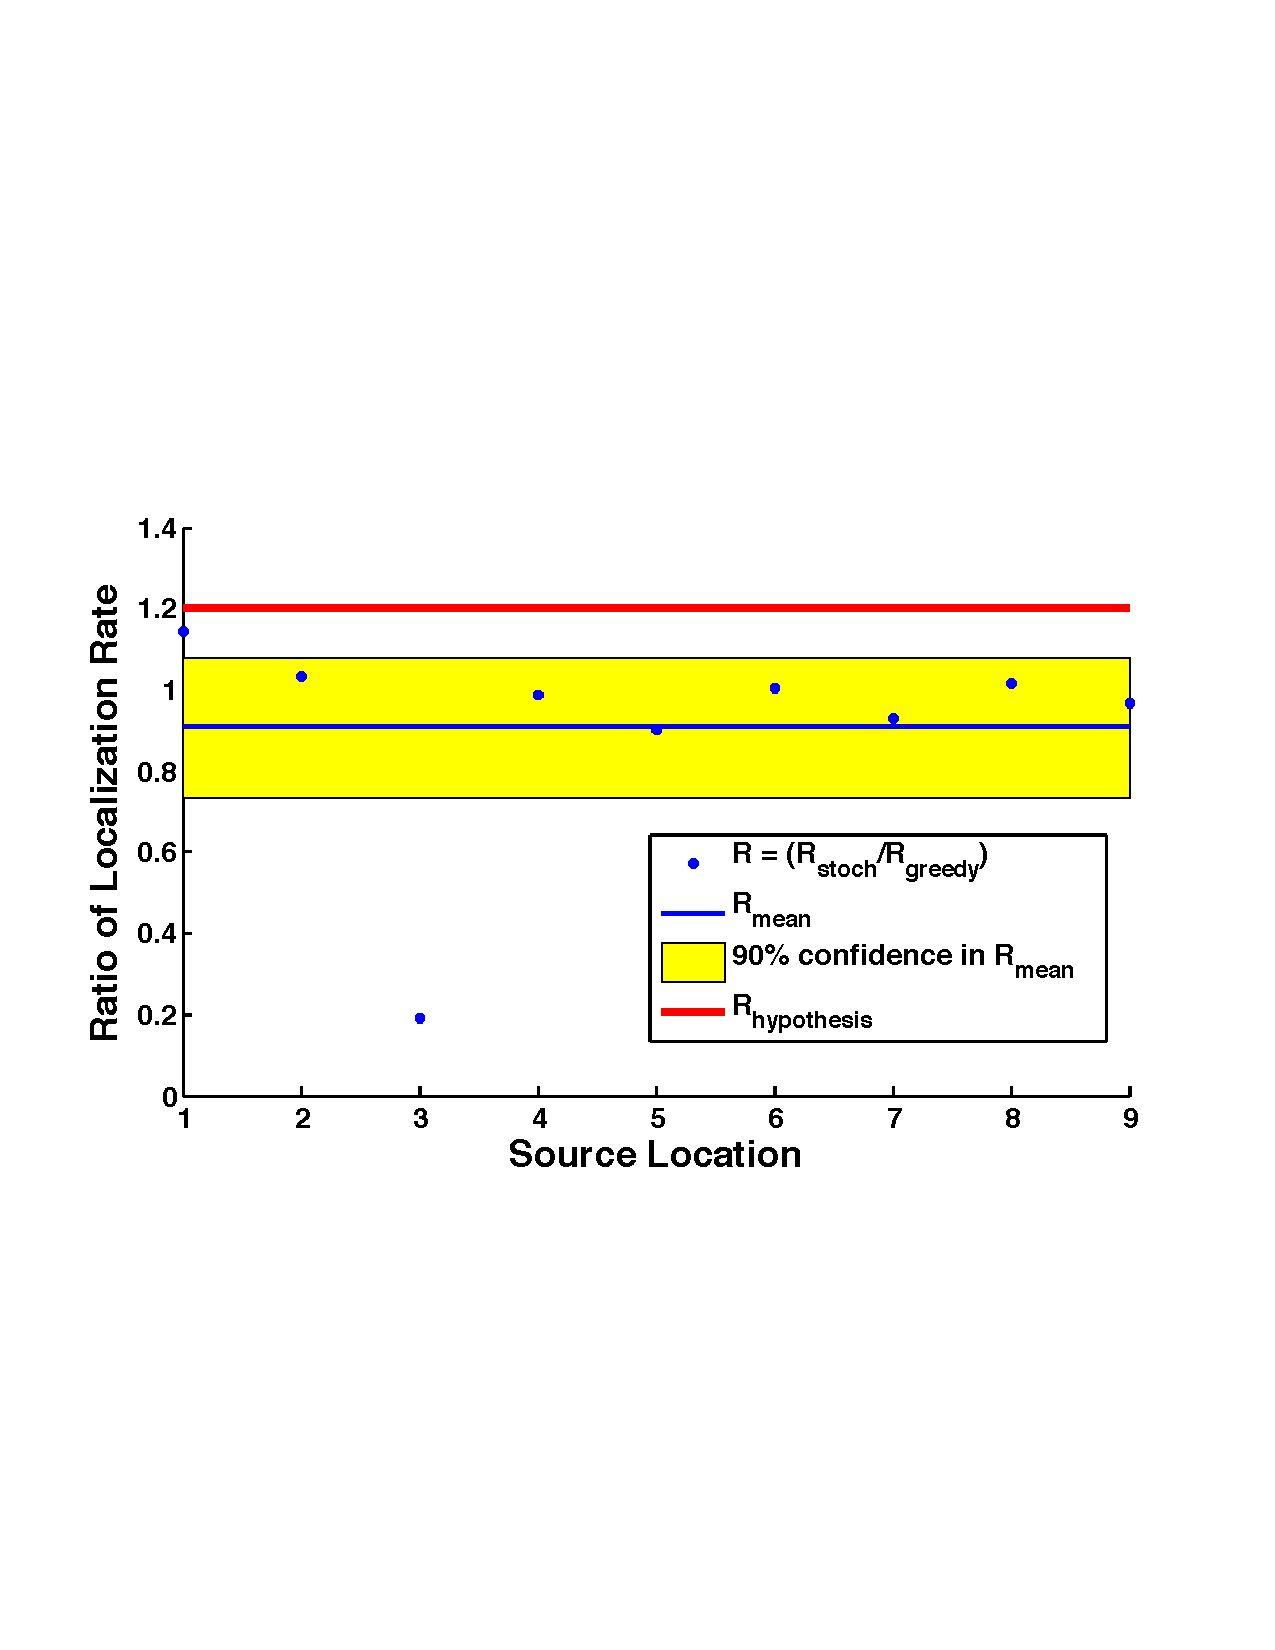
\includegraphics[width=6in]{img/Killer.pdf}}
\caption{Graphical representation of data and hypothesis.}
\label{fig:killer}
\end{center}
\end{figure}


\subsection{Additional Assessment of Results}
\label{sec:additional}
In addition to the assessment of the hypothesis presented in section \ref{sec:hos}, a two-sided Student's
t-test with 8 degrees of freedom was used on the hypothesis $R_{mean}
= 1$ to determine whether there was any statistically significant
difference in the mean localization rates using the two planners.  This test gave
a t-statistic of $-1.0903$ and a p-value of $0.3073$, showing that
there is no statistically significant difference in the mean localization
rate achieved with the stochastic planner and the rate achieved with
the simple gradient descent planner.

\section{Discussion}
\label{sec:discussion}
As described in the previous section, the stochastic planner was not
shown to produce a higher mean localization
rate than the simple gradient descent planner.  One possible cause may
have been
that the system did not produce a statistically significant increase
in the sum of probability mass inside the localization radius using
either planner.  The results of a two-sided Student's t-test on the
null hypothesis $\frac{m_f}{m_0} = 1$ are given in Table
\ref{tab:nofind}.  Although the t-statistics show some increase in the
sum of probability mass inside the localization radius,
particularly in the case of the stochastic planner, this increase is
not significant at a 10\% level.

\begin{table}[htb]
\begin{center}
\begin{tabular}{|c||c|c|}
\hline
& t-statistic & p-value \\
\hline \hline
Greedy Planner & 1.0296 & 0.3333\\
\hline
Stochastic Planner& 1.3994 &0.1993\\
\hline
\end{tabular}
\caption[Student's t-test on probability mass increase inside
localization radius.]{Student's t-test for an increase in the sum of probability
  mass inside the localization radius over the time of a trial.
  These results show no statistically significant increase.}
\label{tab:nofind}
\end{center}
\end{table}


One reason that the probability mass inside the localization
radius was not shown to increase over the time of a trial may have been
the presence of air currents in the room due to the ventilation
system, the motion of the robot, and other random disturbances. Currents may have invalidated the
assumption that the air directly above the true source location
holds a higher chemical vapor concentration than all surrounding
points.  A qualitative drifting behavior was observed in carrying out
the experiment, where higher concentration measurements were taken
at a distance of one to two meters in one direction from the source than were
taken at similar distances in other directions, and even at the exact
source location.  Further experimental characterization of indoor
chemical dispersion is necessary to confirm this drifting
behavior quantitatively.  The robotic localization system tested in
this experiment attempts to localize the area of highest
concentration, since the estimation algorithms assume the area of highest
concentration to be the location of the true source.  If the true
source location is in fact different from the location of the
highest chemical vapor concentration, the system may not be able to accurately
localize the source, regardless of which planner is used.  The
possibility of system failure in the manner described represents a lack of robust estimation techniques, and
calls for further research in the area of estimation algorithms for
indoor robotic odor localization.

The stochastic planner was expected to produce a greater localization
rate than the simple gradient descent planner due to the fact that it
was expected to gather concentration measurements from a larger
percentage of the test room area.  In experimental trials with the
stochastic planner, the system did gather measurements from a larger
area than in trials with the greedy planner.  This result is shown
qualitatively by the comparison of robot paths in Figure \ref{fig:paths} and
quantitatively in Table \ref{tab:paths}, where $A_{greedy}$ and
$A_{stoch}$ are the percentage of the area of the test room ``covered''
using the greedy planner and the stochastic planner respectively.  For
the purpose of this analysis, the covered area is calculated by the
area of the convex hull
of the set of locations at which the robot took measurements, i.e., the area of
the smallest convex shape that includes all of the measurement locations.

\begin{figure}
\begin{center}
\fbox{
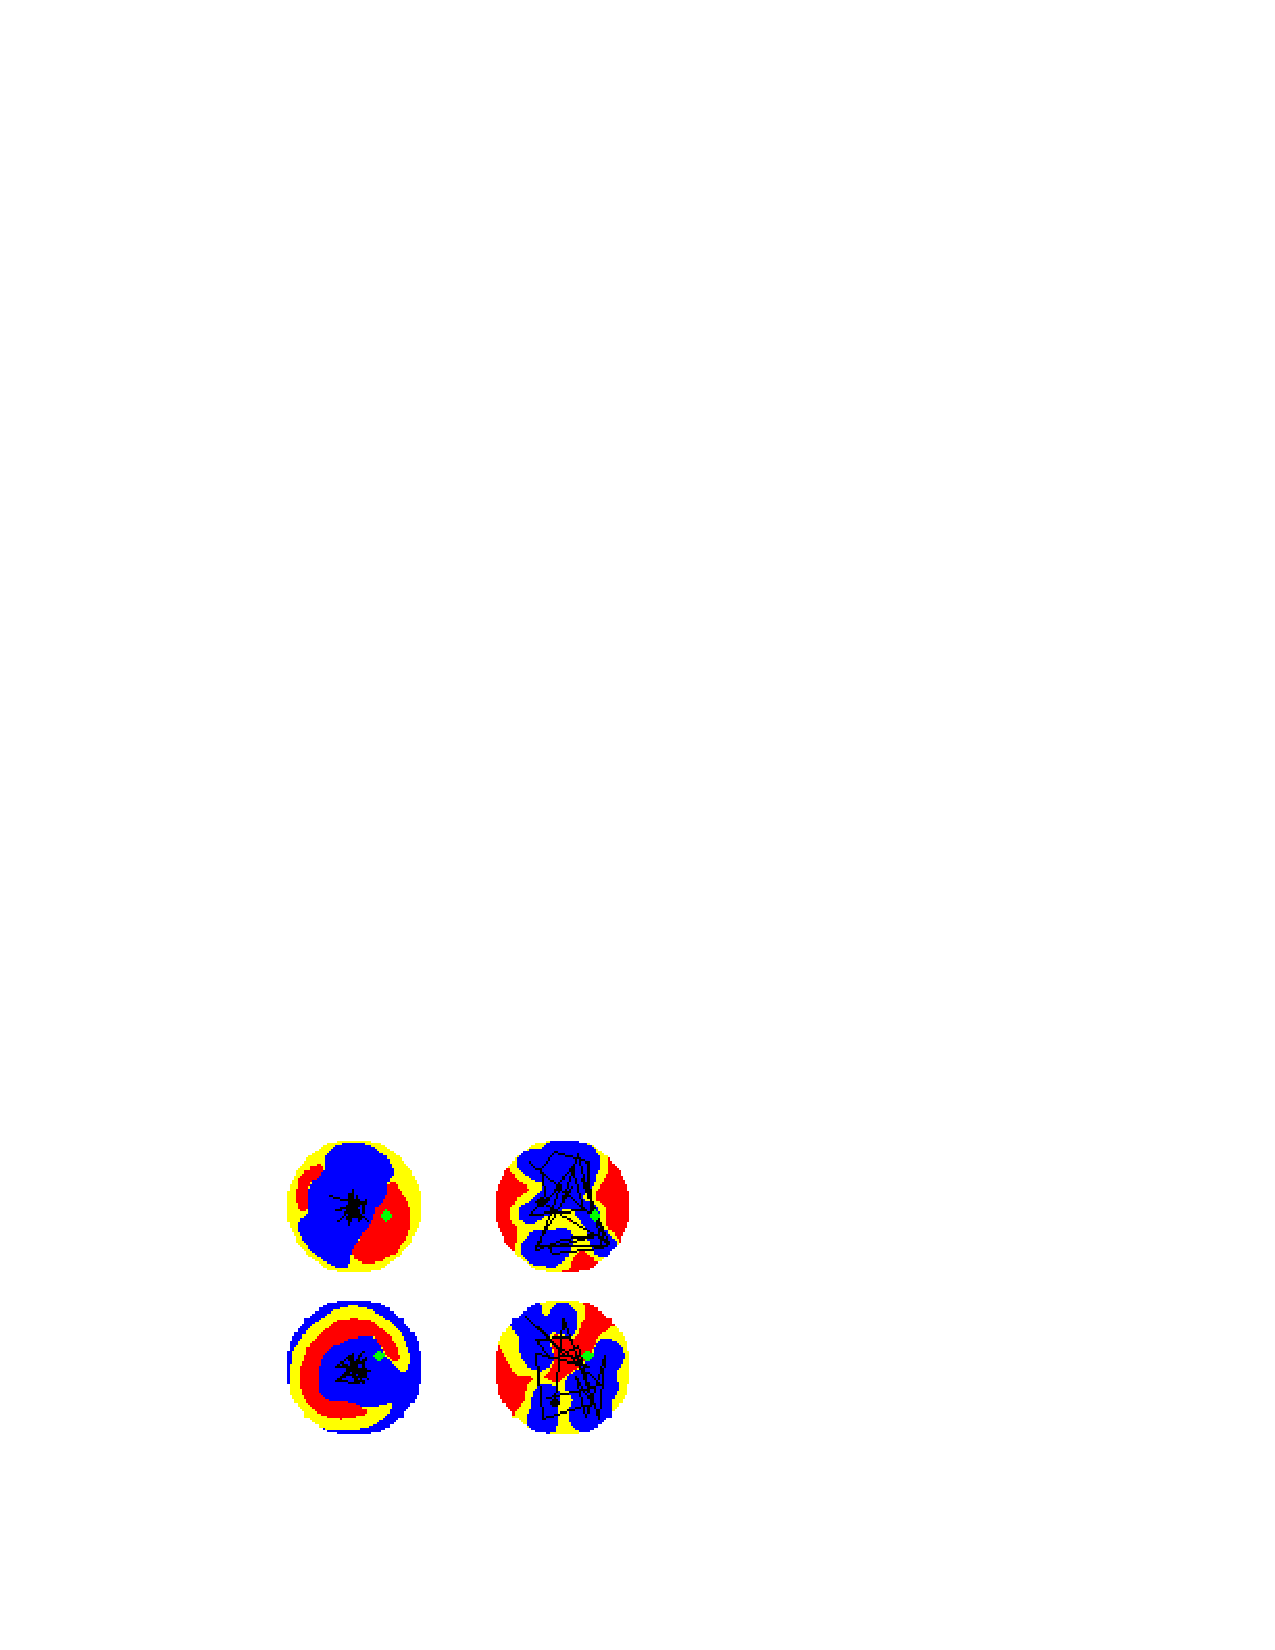
\includegraphics[width=6in]{img/paths.pdf}}
\caption[Final posterior estimates for source locations 7 and 8]{Comparison of robot paths and resulting final particle filter
  probability distributions using the greedy planner (left) and the
  stochastic planner (right) for source locations 7 (top) and 8 (bottom). The
  robot paths are shown in black, where each corner represents a
  measurement location, and the true source locations are
  shown in green.  The circular color fields represent the particle
  filter probability distributions.  The particles making up the top 25\% of the
  probability mass is shown in red, the particles making up the next
  25\% are shown in yellow, and the bottom 50\% are shown in blue. It
  is clear that the different planners produce different distributions
of measurements over the space in the test room, and this results in
different final particle filter probability distributions.}
\label{fig:paths}
\end{center}
\end{figure}

\begin{table}[htb]
\centering
\resizebox{\columnwidth}{!}{
\begin{tabular}{|c||c||c||c||c||c||c||c||c||c|}
\hline
 Source Location & 1 & 2 & 3 & 4 & 5 & 6 & 7 & 8 & 9 \\
\hline \hline
$A_{greedy}$ & 0.1006 & 0.0750 & 0.237 & 0.0775 & 0.0802 & 0.1042 & 0.0669 & 0.0561 & 0.0612 \\
\hline
$A_{stoch}$ & 0.4940 & 0.4523 & 0.5405 & 0.5278 & 0.5032 & 0.5717 & 0.4930 & 0.5469 & 0.5311 \\
\hline
\end{tabular}}
\caption{Fraction of possible area covered by the different planning algorithms.}
\label{tab:paths}
\end{table}

The differences in the area over which concentration measurements were
taken using the greedy planner and the stochastic planner caused the
two planners
to produce different final particle filter probability distributions,
as illustrated qualitatively in Figure \ref{tab:paths}.  However, as
discussed in section \ref{sec:results}, the difference in final
probability distributions did not produce a statistically significant
difference in the localization rate.  In the case where the true source location is
not the point of highest concentration, as discussed earlier in this section, the use of a localization radius about
the true source location
to determine the localization rate may not fully characterize
differences in the performance of the two planners.  Though the use of a
localization radius accurately
assesses the performance of the system in localizing the true source,
and thus correctly and accurately assesses the hypothesis, this metric only takes
into account a subset of the information gained by the particle filter
during a trial.

It is feasible that a more robust estimaton technique could be developed through
future research that takes into account the fact that a maximum in the
chemical vapor concentration field may not exist at the true source
location.  In this case, a preliminary analysis of the
differences in performance of the greedy planner and the
stochastic planner that is not entirely obscured by the assumption of a chemical
concentration maximum at the true source location may prove useful.  A
metric that consists of calculating a
weighted average distance from each particle location to the true
source location was chosen.  The weight of each particle was equal to the
probability mass held by that particle.  The weighted average distance
of the final posterior of each trial from the true source location is
presented in Table \ref{tab:weighted-distance}.  $D_{greedy}$ is the final
weighted average distance using the greedy planner, and
$D_{stoch}$ is the final weighted average distance using the
stochastic planner for each source location.  The ratio
$\frac{D_{stoch}}{D_{greedy}}$ is also presented as a comparison
between the two planners.  A two-sided Student's t-test on the
hypothesis $\frac{D_{stoch}}{D_{greedy}} = 1$ gave a t-statistic of
$0.8862$ and a p-value of $0.4014$, and thus the ratio is not
statistically significantly different from 1.  However, if source
location 3 is ignored on grounds that the trial with the greedy
planner for this location localizes the source an order of magnitude
more effectively than any of the other trials, and thus dominates the results as shown in
Table \ref{tab:data}, the same test
gives a t-statistic of $-2.4529$ and a p-value
of $0.0439$.  This means that for the trials that seem not to
localize the source, the stochastic planner may gain more information
about the location of the true source than the greedy planner with
statistical significance.

\begin{table}[htb]
\centering
\resizebox{\columnwidth}{!}{
\begin{tabular}{|c||c||c||c||c||c||c||c||c||c|}
\hline
 Source Location & 1 & 2 & 3 & 4 & 5 & 6 & 7 & 8 & 9 \\
\hline \hline
$D_{greedy}$ & 3.0630 & 4.5139 & 2.1940 & 3.9041 & 3.8425 & 3.2819 & 3.5805 & 3.4443 & 4.0892 \\
\hline
$D_{stoch}$ & 3.0180 & 4.4869 & 3.0832 & 3.9119 & 3.8311 & 3.2875 & 3.5517 & 3.4059 & 4.0805 \\
\hline
$\frac{D_{stoch}}{D_{greedy}}$ & 0.9853 & 0.9940 & 1.4053 & 1.0020 & 0.9971 & 1.0017 & 0.9920 & 0.9888 & 0.9979 \\
\hline
\end{tabular}}
\caption[Probabilistically weighted distance from the posterior estimate to the
source location]{Weighted distance of the posterior particle distribution from the true
  source location. The weighted distance is the average of the distances from
  each particle location to the source location weighted by the probability
  mass of the posterior held by that particle.}
\label{tab:weighted-distance}
\end{table}


One non-ideal characteristic of the weighted average distance metric
is that the particles far from the true source location have a greater
impact on the result than particles close to the source location.
The Kullback - Leibler divergence (KL divergence) of the final estimator
probability distribution from an ``ideal'' Gaussian posterior about
the true source location for each trial is shown in Table
\ref{tab:kl-ideal}.  The KL-divergence metric does not allow particles far from
the source to be of greater impact than particles close to the source
like the weighted average distance metric does.  A
two-sided Student's t-test on the hypothesis
$\frac{KL_{stoch}}{KL_{greedy}} = 1$, excluding source location 3, gives a t-statistic of -0.3539 and
a p-value of 0.7338.  Thus, the ratio $\frac{KL_{stoch}}{KL_{greedy}}$
is not statistically significantly different from 1, even without the
third source location data.  This result supports the claim that the
stochastic planner may be better than the greedy planner at decreasing the probability mass of
particles far from the true source location.  The claim makes
intuitive sense since the stochastic planner allows the robot to cover
more of the test room, as discussed earlier in this section.  The
observation that the stochastic planner may be better than the greedy
planner at decreasing the probabilities of particles far from the true
source location may be prove valuable in future research on robust
estimation and planning techniques for robotic odor localization.


\begin{table}[htb]
\centering
\resizebox{\columnwidth}{!}{
\begin{tabular}{|c||c||c||c||c||c||c||c||c||c|}
\hline
 Source Location & 1 & 2 & 3 & 4 & 5 & 6 & 7 & 8 & 9 \\
\hline \hline
$KL_{greedy}$ & 1.3819 & 1.8294 & 0.6025 & 1.4937 & 1.4636 & 1.3319 & 1.3668 & 1.3803 & 1.5682 \\
\hline
$KL_{stoch}$  & 1.2861 & 1.7989 & 1.2882 & 1.5312 & 1.5107 & 1.3297 & 1.3736 & 1.3431 & 1.5974 \\
\hline
Ratio $\frac{KL_{stoch}}{KL_{greedy}}$ & 0.9306 & 0.9833 & 2.1381 & 1.0251 & 1.0322 & 0.9984 & 1.0050 & 0.9730 & 1.0186 \\
\hline
\end{tabular}}
\caption{Kullback-Leibler divergence of the final particle filter
  posterior distribution from an 'ideal' Gaussion posterior distribution . }
\label{tab:kl-ideal}
\end{table}


%  it was desired to know
% whether there was any difference between the full amount of information
% gained in a trial using the greedy planner, and the amount gained
% using a stochastic planner.  The amount of information gained in each
% trial was measured by calculating the Kullback – Leibler divergence (KL
% divergence) of
% the final particle filter probability distribution from the initial
% uniform distribution where all of the particles are assigned the same
% probability.  The KL divergence of the particle filter probability
% distribution in each trial is shown in Table \ref{tab:allinfo}.

% \begin{table}[htb]
% \centering
% \resizebox{\columnwidth}{!}{
% \begin{tabular}{|c||c||c||c||c||c||c||c||c||c|}
% \hline
%  Source Location & 1 & 2 & 3 & 4 & 5 & 6 & 7 & 8 & 9 \\
% \hline \hline
% $KL_{greedy}$  & 0.0029 & 0.0019 & 0.3156 & 0.0024 & 0.0071 & 0.0007 & 0.0070 & 0.0039 & 0.0085 \\
% \hline
% $KL_{stochastic}$ & 0.0013 & 0.0082 & 0.0017 & 0.0015 & 0.0030 & 0.0019 & 0.0012 & 0.0008 & 0.0011 \\
% \hline
% $\frac{KL_{stoch}}{KL_{greedy}}$ & 0.4463 & 4.3945 & 0.0052 & 0.6107 & 0.4157 & 2.7365 & 0.1711 & 0.1990 & 0.1282 \\
% \hline
% \end{tabular}}
% \caption[KL divergence of posterior distribution from a uniform distribution]{Kullback-Leibler divergence of the final particle filter
%   probability distribution from the initial uniform particle
%   probability distribution.  This is a measure of how much
%   information about the environment was gained by the system in each trial. }
% \label{tab:allinfo}
% \end{table}

% The mean of the ratios $\frac{KL_{stoch}}{KL_{greedy}}$ over the 9
% source locations is equal to $mean(\frac{KL_{stoch}}{KL_{greedy}}) =
% 1.0119$.  A two-sided Student's t-test with the null hypothesis
% $mean(\frac{KL_{stoch}}{KL_{greedy}}) = 1$ gave a t-statistic of
% $0.0235$ and a p-value of $0.9818$.  This shows there is no significant
% difference in the information gain between the two.

% The important metric is not general information gain, however, but is the gain
% of information about the source location. There are other metrics that use the
% information from all of the particles to measure how well the source location
% has been estimated. 

% Table \ref{tab:weighted-distance} shows the probabilistic weighted distances
% of the true source location to the posterior estimate.  The weighted distance is
% calculated by taking the weighted average distance from each particle location
% to the source location, where the weighting for each particle is determined by the
% probability mass held by the particle at the end of a trial.  A two-sided
% Student's t-test on the ratio of the stochastic to the greedy weighted distance
% shows that the ratio is not statistically significantly different from 1,
% resulting in a t-statistic of $0.8862$ and a p-value of $0.4014$. If, however,
% we look at all the source locations where one of the planners did not
% definitively find the source, i.e. all the source locations other than source
% location 3, the ratio of the weighted distances is significantly different from
% 1. Running the same Student's t-test over the other 8 source location gives a
% t-statistic of $-2.4529$ and a p-value of $0.0439$. This is statistically
% significant difference from 1 at the $5\%$ level. This difference is not
% overwhelming, as the mean ratio of the weighted distances is $0.9948$, but at a
% minimum this shows that by covering more of the search space the stochastic planner
% lowers the probability of more areas being potential source locations.


\subsection{Future Work}
As discussed in section \ref{sec:discussion}, one reason that the
experimental results did not show a statistically significant
difference in the localization rates using the
greedy planner and the stochastic planner was the lack of statistically significant
difference between final and initial sums of probability mass within
the localization radius.  The suspected cause of this lack of
difference is the use of an inadequate estimation technique.  It is
believed that further research in the area of probabilistic estimation for robotic
odor localization is necessary before additional research in the area
of planners will be meaningful.

There are many avenues for improvements to estimation. The simplest would
require only choosing parameters for the current estimator. The data collected
while running the trials can be combined into a much larger dataset than the
preliminary one that was used to fit parameter values for the measurement model.
Additionally, the value for the measurement noise, $\sigma$ in Table
\ref{tab:estimator-parameters}, was set to a value an order of magnitude larger
than the value the initial fitting indicated, because in the preliminary trials
the original sigma value caused the probability estimate to collapse too quickly
to the wrong source location. As the results in Table \ref{tab:nofind} show,
over the course of the trials the probability mass did not change in a
statistically significant manner, meaning that the posterior estimate was likely
too slow in collapsing.  If the posterior was indeed too slow to collapse, the
measurement noise should be set to a smaller value. 

Rigorous characterization of the sensor dynamics could also lead to a more
effective measurement model. As previously noted, the baseline value of sensor
readings changed significantly across testing days. Understanding and accounting
for the factors that caused these changes could improve the performance of the
estimator. It was also observed that the sensor would take 20 to 30 minutes
beyond the time necessary for the sensor chamber to heat to the proper
temperature for the readings stabilize at a baseline value. Understanding and
characterizing this behavior, along with any other potential time-varying
behavior of the sensor, could again improve estimator performance. Finally, an
accurate mapping from sensor readings to chemical concentrations could be
necessary for more sophisticated measurement models.  This mapping could be
experimentally determined by recording sensor readings over time while the sensor
is exposed to a known concentration level. This could be achieved in a small, sealed
container inside of which a known quantity of ethanol could be allowed to
evaporate. 

Dispersion dynamics holds the widest range of potential estimation
improvements, though many of these improvements are perhaps more difficult to
implement than the improvements mentioned previously.  The likelihood function
is based on a model of diffusion, but as discussed in Section
\ref{sec:lit-review}, the effect of convection dominates that of diffusion for
chemical dispersion in an indoor environment. There are many ways to incorporate
convective effects into the measurement function, covering a large range in
degree of difficulty. The most accurate description of the system would likely
require methods of computation fluid dynamics dependent on knowledge of the room
shape and ventilation locations. These computations, however, would likely be
too resource intensive to run in real-time on a robotic platform, and the
dependence on location specific features potentially loses generality of the
solution. The latter objection could be addressed by integrating the dispersion
model with online mapping, but this would greatly increase the complexity of the
solution. Simpler options should likely be exhausted before turning to
computational fluid dynamics tools.

Simpler models similar to that used in the conducted experiment could still
reflect that convection is the dominant dispersive effect. For instance, with
convection being dominant we expect dispersion to be characterized by small
pockets of high concentration, with these pockets most common and dense near the
source, and then becoming less common and less dense farther from the source.
This would lead to rapidly changing, high variance readings near the source
location, where many dense concentration packets quickly pass over the mouth of
the sensor, and slower changing, lower variance readings farther from the source
location. This type of behavior was observed by this experiment, and by Ferri
et. all in their experiments. \cite{ferri} Considering of this behavior, in
additional to the average reading value a measurement model could predict the
variance of sensor readings, or speed of the change in readings, based on
the distance of the robot from the source.


\section{Summary and Conclusion}
The data collected does not find any statistically significant evidence that a
stochastic planner localizes a chemical source at a faster rate that a greedy
gradient descent planner. It is believed that potential difference in the planning
algorithms' performances were masked by failures of the estimation techniques.
Further research into robust estimation techniques for indoor robotic odor
localization is needed to advance the field.

\section{Acknowledgments}
We, the authors, would like to thank our faculty advisors, Professors Youssef
Marzouk and Nicholas Roy, for the expertise and experience they brought to the
project, and all the time they invested in teaching us and brainstorming with
us. We would like to thank Josh Joseph and Javier Velez for always being happy
to make time to help us work through the issues we faced, and for being so
patient and understanding while explaining new concepts and techniques to us.
Xun Huan and Sachi Hemachandra also volunteered their time to help us progress
through the project. Finally, we must thank the 16.62x course staff: Professors
Brian Wardle, Edward Greiter, and Sheila Widnall, communications instructor
Jennifer Craig, laboratory instructors Dick Perdichizzi, Dave Robertson, and Tod
Billings, and teaching assistant Louis Perna. The course staff was determined to
help us successfully complete our project, and help push us through to the
finish line. Without the guidance of all those who helped us on this project, we
would have never have been able to complete it.


\newpage
\bibliographystyle{aiaa}
\bibliography{sources}
\nocite{*}

\newpage
\appendix
\section{Additional Figures}
\begin{figure}
\begin{center}
\fbox{
\includegraphics[height=5.9in]{img/all-posteriors.pdf}}
\caption[Final posterior estimates for all trials]{
  Robot paths and resulting final posterior
  probability estimates using the greedy planner (left) and the
  stochastic planner (right) for all source locations, with source location 1
  at the top and source location 9 at the bottom. The
  robot paths are shown in black, where each corner represents a
  measurement location, and the true source locations are
  shown in green.  The circular color fields represent the particle
  filter probability distributions.  The particles making up the top 25\% of the
  probability mass is shown in red, the particles making up the next
  25\% are shown in yellow, and the bottom 50\% are shown in blue. }
\end{center}
\end{figure}


\end{document}